% !TeX spellcheck = en_US
\documentclass[french]{yLectureNote}

\title{Mécanique du solide}
\subtitle{Physique}
\author{Paulhenry Saux}
\date{\today}
\yLanguage{Français}

\professor{F.Pettinari}
\usepackage{graphicx}%----pour mettre des images
\usepackage[utf8]{inputenc}%---encodage
\usepackage{geometry}%---pour modifier les tailles et mettre a4paper
%\usepackage{awesomebox}%---pour les boites d'exercices, de pbq et de croquis ---d\'esactiv\'e pour les TP de PC
\usepackage{tikz}%---pour deiffner + d\'ependance de chemfig
% \usepackage{tabularx}%---pour dimensionner automatiquement les tableaux avec variable X
\usepackage{awesomebox}%---Pour les boites info, danger et autres
\usepackage{menukeys}%---Pour deiffner les touches de Calculatrice
\usepackage{fancyhdr}%---pour les en-t\^ete personnalis\'ees
\usepackage{blindtext}%---pour les liens
\usepackage{hyperref}%---pour les liens (\`a mettre en dernier)
\usepackage{caption}%---pour la francisation de la l\'egende table vers Tableau
\usepackage{pifont}
\usepackage{array}%---pour les tableaux
\usepackage{lipsum}
\usepackage{yFlatTable}
\usepackage{multicol}
\newcommand{\Lim}[1]{\lim\limits_{\substack{#1}}\:}
\renewcommand{\vec}{\overrightarrow}
\newcommand{\N}[0]{\mathbb{N}}
\newcommand{\dd}{\mathrm{d}}
\newcommand{\norm}[1]{||\vec{#1}||}
\newcommand{\fo}{\psi(\vec{r},t)}
\newcommand{\foe}{\psi(\vec{r},t)\*}
\newcommand{\HH}{\hat{H}}
\newcommand{\hb}{\hbar}
\newcommand{\lap}{\nabla^2}
\newcommand{\lapcc}{\frac{\partial^2 }{\partial x^2}+\frac{\partial^2 }{\partial y^2}+\frac{\partial^2 }{\partial z^2}}
\begin{document}
\chapter{Cinématique du solide et des solides en contact}
\section{Cinématique du solide}
\subsection{Modèles du solide indéformable}
\subsubsection{Solide indéformable}
\begin{definition}[Solide indéformable]
C'est un solide (S) ``idéal'' dans lequel les atomes sont rigouresuement fixes les uns par rapport aux autres. Tous les points A et B lui appartenant ont une distance constante au cours du temps.
\end{definition}
Ainsi, 3 points situés à des distances fixes forment un solide.
\subsubsection{Point lié à un solide}
\begin{definition}
C'est un point restant à une distance fixe de tous les autres points du solide (S).
\end{definition}
\marginCritical{Il peut se trouver à l'extérieur du solide}.
On le note \(P\in S\)\marginInfo{On note alors la vitesse de \(A\in S\), \(\vec{v}(A\in S/R)\)}. Le centre d’une sphère creuse se déplace comme s’il était lié au solide, mais il n’appartient pas au solide.
\subsubsection{Repère}
SI on définit 4 points O,I,J,K formant un repère, alors R est le repère lié ua solide. On peut associer à tous solide un repère
\subsubsection{Degrès de liberté (DDL)}
\begin{definition}[Degrès de liberté]
Ce sont des coordonnées importantes indépendants qui définissent la position d'un solide dans l'espace au cours du temps
\end{definition}
Ainsi, pour un solide à 3 dimensions, il y a 6 DDL :
\begin{itemize}
\item 3 de translation (x,y,z) pour repérer le centre de masse
\item 3 de rotation (autour des axes) pour l'orientation des autres points du solide par rapport au centre de masse.
\end{itemize}
\subsection{Champ des vitesses dans un solide}
Quand on travaille avec un solide, on considère un ensemble de points. La notion de vitesse d'un solide n'a donc pas de sens et on introduit la notion de champ de vitesse.

Si on considère 2 points A et B, on a \(AB = K\) donc
\begin{flalign*}
\frac{\dd \vec{AB}^2}{\dd t} = 0\\
2 (\frac{\dd \vec{AB}}{\dd t})\cdot \vec{AB} = 0\\
\vec{AB}\cdot (-\vec{v_{A/R}}+\vec{v_{B/R}}) = 0
\end{flalign*}
On obtient
\begin{proposition}[Relation du champ des vitesses dans un solide (Varignon = BABAR)]
\[\vec{AB}\cdot \vec{v_{A/R}} = \vec{AB}\cdot \vec{v_{B/R}}\] qui équivaut à
\[\vec{v_{B\in S/R}} =  \vec{v_{A\in S/R}} + \vec{BA}\wedge \vec{\omega_{S/R}}\] avec \(\vec{\Omega}\) le vecteur rotation du solide par rapport à R.
\end{proposition}
On peut démontrer l'une en fonction de l'autre

\begin{flalign*}
\vec{v_{B\in S/R}} = (\frac{\dd \vec{OB}}{\dd t})_R = (\frac{\dd \vec{OA}}{\dd t})_R + (\frac{\vec{AB}}{\dd t})_R\\
&= \vec{v_{A\in S/R}} + (\frac{\dd \vec{AB}}{\dd t})_{R=S} + \vec{\Omega}_{S/R} \wedge \vec{AB}\\
&= \vec{v_{A\in S/R}} + \vec{0} + \vec{\Omega}_{S/R} \wedge \vec{AB}\\
&= \vec{v_{A\in S/R}}  + \vec{\Omega}_{S/R} \wedge \vec{AB}\\
&= \vec{v_{A\in S/R}}  + \vec{BA} \wedge \vec{\Omega}_{S/R}\\
\end{flalign*}
\subsubsection{Torseur}
On définit le torseur avec un vecteur ``somme'' et un vecteur ``moment''. Le torseur cinématique d'un solide en un point A est \[[V(A/R)] = \vec{\Omega} \vec{v(A\in S/R)} \]. On a \[\vec{Moment}(B) = \vec{Moment(A)} + \vec{BA}\wedge \vec{Resultante}\]
\subsection{Mouvements d'un solide}
\subsubsection{Translation d'un solide}
Un solide S est en translation par rapport à un référentiel R si tous les points de (S) ont m\^eme vitesse par rapport à R ou si \(\vec{\Omega}_{S/R} = \vec{0}\). On peut avoir une translation
\begin{itemize}
 \item uniforme : norme de la vitesse de chacun des points est constante
 \item rectiligne : le vecteur vitesse de tous les points garde une direction constante
 \item circulaire : la trajectoire est un cercle\marginCritical{L'objet ne tourne pas autour de lui-m\^eme mais autour d'un point.}
\end{itemize}
\subsubsection{Rotation d'un solide autour d'un axe fixe}
Un solide s a un mouvement de rotation autour d'un axe fixe par rapport à R s'il existe une droite liée à S dont les points sont fixes par rapport à R. On a alors

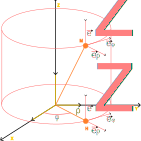
\includegraphics[scale=0.5]{base_c}
\begin{itemize}
 \item \(HA = \rho = OP\)
 \item \(\varphi  = (\hat{\vec{e_x}, \vec{OP}})\)
\end{itemize}
Pour trouver \(\vec{v_{A\in S}}\), on applique Verignon avec \(\vec{\Omega} = \dot{\varphi} \vec{e_z}\). On trouve :
\begin{flalign*}
\vec{v_A} &= \vec{0} - (z\vec{e_z}+\rho \vec{e_{\rho}})\wedge \dot{\varphi}\vec{e_z}\\
&= \rho \dot{\varphi} \vec{e_{\varphi}}
\end{flalign*}
\criticalInfo{Angle orienté}{Il faut bien regarder si la rotation est dans le sens horaire (vitesse angulaire positive) ou antihoraire (vitesse angualire négative)}
\subsubsection{Mouvement général}
Le mouvement le plus général d'un solide associe translation et rotation. Le mouvement de n'importe quel point \(B\in S\) sera défini à partir de la connaissance de la vitesse d'un autre point de S
\checkInfo{Exemple en deux dimensions}{
\includegraphics[scale=0.5]{exemple2}

On a \(l = OA = AB\) et \(\varphi_1 = \hat{\vec{e_x}, \vec{OA}}\) et \(\varphi_2 = \hat{\vec{e_x}, \vec{AB}}\) et \(\beta = \hat{\vec{OA}, \vec{AB}}\). De plus, \(\vec{\Omega_{OA}} = \cdot{\varphi_1}\vec{e_z}\) et  \(\vec{\Omega_{AB}} = \cdot{\varphi_2}\vec{e_z}\) Il faut toujours prendre la vitesse angulaire par rapport à un axe fixe.

En se plaçant dans 2 bases orthonormées, on veut déterminer \(\vec{v_{A/R}}\) et  \(\vec{v_{B/R}}\).

Donc, avec Verignon
\begin{flalign*}
\vec{V_A/R} &= \vec{A\in OA/R} = \vec{v_{A\in AB/R}}\\
&= \vec{v_{O\in OA/R}} + \vec{AO}\wedge \vec{\Omega}_{OA/R}\\
&= -l \vec{e_{\rho}}\wedge \dot{\varphi_1} \vec{e_z}\\
&= l\dot{\varphi_1}\vec{e_{\varphi_1}}
\end{flalign*}
puis

\begin{flalign*}
\vec{v_{B\in AB/R}} &= \vec{A\in OA/R} + \vec{BA}\wedge \vec{\Omega}_{AB/R}\\
&= l\dot{\varphi_1}\vec{e_{\varphi_1}} - l\vec{e_{\rho_2}}\wedge \dot{\varphi_2}\vec{e_z}\\
&= l\dot{\varphi_1}\vec{e_{\varphi_1}} + l\dot{\varphi_2}\vec{e_{\varphi_2}}
\end{flalign*}
}
\section{Cinématique des solides en contact}
\subsection{Introduction}
On considère 2 solides se déplaçant par rapport à R en restant en contact permanent entre eux. On suppose que le contact est ponctuel et s'effectue au point I. On distingue en I :
\begin{itemize}
 \item Le point géométrique I
 \item Le point matériel \(I_1\in S_1\)
 \item Le point matériel \(I_2\in S_2\)
\end{itemize}
Ces derniers sont confondus à l'instant t.
\checkInfo{Disque (S1) roulant sur un plan (S2) }{
\includegraphics[scale=0.5]{exemple3}

Si on utilise \(\vec{v_{I/R}} = (\frac{\dd \vec{OI}}{\dd t})_R = \frac{\dd}{\dd t}(x\vec{e_x}) = \dot{x}\vec{e_x}\), on a la vitesse du point géométrique.

Pour déterminer \(\vec{v_{I_1\in S_1}} = \vec{v_{C\in S_1/R}} + \vec{I_1C}\wedge \omega \vec{e_z} = \dot{x}\vec{e_x} - r \omega \vec{e_x}\).

On a donc \(\vec{v_{I_1}} = (\dot{x}-r\omega)\vec{e_x} \neq \vec{v_I} \neq \vec{v_{I_2\in sol}}\)
}
\subsection{Vitesse de glissement}
\begin{definition}[Vitesse de glissement]
Notée \(\vec{v_g}\), elle est définie par \[\vec{v_{g1/2}} = \vec{v_{I_1\in S_1/R}} - \vec{v_{I_2\in S_2/R}}\]
\end{definition}
\subsection{Condition de roulement sans glissement}
\begin{definition}[CRSG]
Elle correspond à \(\vec{V_g} = 0\). On a alors \(\vec{v_{I_1\in S_1/R}} = \vec{v_{I_2\in S_2/R}}\)
\end{definition}
\checkInfo{Disque}{
On a vu que \(\vec{V_{I_1}} = (\dot{x}-r\omega), \vec{I_2} = \vec{0}\). On en déduit que pour se trouver en CRSG, il faut que \(\dot{x} = r\omega\)
}
\section{Mouvement plan d'un solide}
\subsection{Mouvement plan}
\begin{definition}[Mouvement plan]
C'est un mouvement tel que chaque point du solide S se déplace dans un plan parallèle à un plan fixe Q dans le référentiel R
\end{definition}
C'est le cas d'un cylindre tournant autour de lui-m\^eme. Un mouvement est plan dans le cas où les actions mécaniques\marginTips{On peut avoir la somme des forces qui vaut 0 mais avoir quand m\^eme un mouvement (avec des forces opposées mais s'exerçant sur des c\^otés opposés du solide.)} et vitesses initiales sont contenues dans le plan. L'étude du mouvement de S se réduit à l'étude de la section dans le plan Q\marginTips{En général la section contenant le centre de masse}.
\subsection{Centre instantané de rotation (CIR)}
\begin{definition}[CIR]
On appelle CIR du plan Q' (plan invariablement lié à la section du solide (S) par Q) à l'instant t le point I du solide (S) dont la vitesse par rapport à R est nulle. On a donc \[\vec{v_{i\in  S}} = \vec{0}\]
\end{definition}
\checkInfo{Exemple}{
Le point $I_1$ de contact d'un cerceau sur un sol fixe lorsque le solide est en CRSG est un exemple. En effet, ce dernier a bien une vitesse nulle par la CRSG.

On peut aussi trouver le CIR d'une échelle contre un mur.

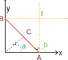
\includegraphics[scale=0.5]{exemple4}

On a \(\Omega = \dot{\beta}\vec{e_z} = -\dot{\alpha}\vec{e_z}\) car \(\beta  = \pi-\alpha\). On cherche le CIR qui vérifie \(\vec{v_{I\in S}} = \vec{0}\). On a
\begin{flalign*}
\vec{v_a} = \vec{v_I} + \vec{AI}\wedge \vec{\Omega}\\
\vec{v_b} = \vec{v_i} + \vec{BI}\wedge \vec{\Omega}
\end{flalign*}

Comme on sait que \(\vec{v_a}\) est selon \(\vec{e_x}\) et \(\vec{v_b}\) selon \(\vec{e_y}\), on en déduit que \(\vec{AI}\) est selon \(\vec{e_y}\) et \(\vec{BI}\) selon \(\vec{e_x}\) (en prenant en compte que \(\vec{\Omega}\) est selon \(-\vec{e_z}\))

Ici, ce point I n'est pas le point géométrique.%Expliquer pourquoi

La vitesse est en effet de \(2l\dot{\alpha}(\dots)\).
}
Il y a souvent une équivalence entre les 2 notions
\chapter{Éléments cinétiques des solides}
\section{Centre de masse}
On considère un solide qui correspond à uen distribution continue de points matériels. La masse est définie par \[M = \int\int\int \rho(A)\dd V\] si le solide est un volume avec A un point quelconque de S et \(\rho(A)\) une masse volumique autour de A.
\subsection{Centre de masse}
\begin{definition}[Centre de masse ou centre d'inertie]
Noté C ou G, il est défini par \[M\vec{OC} = \int_{S} \vec{OA}\cdot \dd m = \int_V \vec{OA} \cdot \rho(A)\dd V\]
Il correspond au barycentre des points matériels affectés de leur masse respective : \[\int_S \vec{CA}\dd m = \vec{0}\]
\end{definition}
La première expression permet de déterminer les coordonnées de C. Il ne faut pas confondre centre de masse et centre d'inertie et centre de gravité\marginTips{Le centre de gravité est confondu avec le centre de masse uniquement si le champ de gravitation uniforme.}
\subsection{Propriétés}
\subsubsection{Symétries du système}
Le centre de masse respecte les symétries du système. Si il existe un élément de symétrie (plan, centre, axe), ce dernier contient le centre de masse.
\subsubsection{Associativité du centre de masse}
Lorsqu'un solide est constitué de l'association de plusieurs solides, le centre de masse correspond au barycentre des centres de masse de chaque solide affecté de leur masse respective. Ainsi \[M\vec{OC} = \sum_i m_i \vec{OC_i}\] Il s'agit d'une somme algébrique qui contient un signe négatif dans le cas d'un trou.\marginCheck{Par exemple, dans le cas d'un disque évidé d'un autre disque, on peut faire la somme du premier disque moins celle du second disque}
\subsubsection{Théorèmes de Guldin}
Ils permettent de déterminer rapidement les positions du centre de masse de courbes ou de surfaces matériels simples.
\subsection{Exemples}
\subsubsection{Part de tarte}%polycopié
\subsubsection{Centre de masse d'un c\^one homogène}%polyco
On considère un c\^one crux de densité surfacique \(\sigma\) et d'élément de surface \(\dd S\)

On définit la hauteur di c\^one \(h\) et \(\alpha\) l'angle du cone à partir du sommet. On sait par symétrie que le cdm se trouve sur l'axe perpendiculaire à la base et passant par le sommet. Reste à savoir où il se trouve sur l'axe \(Oz\).

\begin{flalign*}
Mz_C = \int\int\int_S \dd m z
\end{flalign*}
On prend \(\dd S = \rho\dd \varphi\dd l\) avec \(\rho = z\tan(\alpha) = \frac{\rho}{h}, l = \frac{z}{\cos(\alpha)}\), donc \(\dd l = \frac{\dd z}{\cos(\alpha)}\).

Donc
\begin{flalign*}
M\cdot z_c &= \int\int\sigma \dd S\cdot z = \sigma \int_0^{2\pi}\int_0^{h}\rho\dd \varphi \dd l \cdot z\\
&= \sigma\int_0^{2\pi}\dd \varphi\int_0^hz\frac{\rho}{h}\frac{\dd z}{\cos(\alpha)}\\
&= \sigma 2\pi \frac{\rho}{h}\frac{1}{\cos(\alpha)}\frac{h^3}{3}\\
M &= \int\int\sigma \dd S\\
&= 2\pi\sigma \frac{\tan(\alpha)}{\cos(\alpha)}\frac{h^2}{2}\\
z_c &= \frac{2}{3}h
\end{flalign*}
\section{Moment d'inertie}
\subsection{Par rapport à un axe}
\begin{definition}[Moment d'inertie]
C'est la quantité \[I_{\Delta} = \sum_i d_i^2 = \sum_i m_i\vec{H_iA_i}^2\] avec \(H_i\) le projeté orthogonal de \(A_i\) selon l'axe \(\Delta\)
\end{definition}
Pour un solide, on a \[I_{\Delta} = \int\int\int_S \vec{HA}^2 \rho \dd V = \int\int\int \vec{HA}^2 \dd m\]

Le moment d'inertie est un obstacle au mouvement circulaire autour de l'axe. Le moment d'inertie a la dimension d'une masse multipliée par une distance au carrée.
\subsection{Méthode de calcul}
\subsubsection{Systèmes avec symétrie de révolution}
On étudie le cas d'un cylindre creux ou plein et d'un disque ou cerceau. Dans les 2 cas, l'axe Oz est l'axe de symétrie de révolution. Pour des raisons de symétrie, les moments d'inertie \(I_{ox}\) et \(I_{oy}\) sont les m\^emes. Ainsi\marginCritical{Savoir redémontrer jusqu'à l'apparyion de \(I_{oz}\)} \[I_{ox} = \int_V (y^2+z^2)\dd m\]
\[I_{oy} = \int_V (x^2+z^2)\dd m\]
\[I_{ox}+I_{oy} = \int_V (y^2+x^2)\dd m + 2\int z^2\dd m = I_{oz} + 2\int z^2\dd m\]

Cas du cercle : \(z = 0, x^2+y^2 = R^2, \dd  m \lambda \dd l =\lambda R \dd \varphi \).
Donc \(2I_{ox} = I_{oz} = \int R^2 \lambda R \dd \varphi \dd R = \lambda R^2 2 \pi\) et \(M = \int \dd m = R\lambda 2\pi\), donc \(I_{oz} = MR^2\)\marginWarning{Résultat à savoir}.

Cas du disque : On a toujours \(z=0, x^2+y^2 = r^2, \dd m = \sigma \dd S\). On a aussi \(I_{ox} = \int_{0}^{2\pi}\int_0^R r^2\sigma r\dd \varphi\dd r = \sigma 2\pi \frac{R^4}{4}\) avec \(M = \int \sigma \dd S = \sigma \pi R^2\), donc \(I_{oz} = 2I_{oy} = M\frac{R^2}{2}\).
 \end{document}
